\documentclass[fleqn,10pt]{wlscirep}
\usepackage[utf8]{inputenc}
\usepackage[T1]{fontenc}
\usepackage{booktabs}

\title{Bridging international search interest and local news: a content-based recommender for Bosnian natural-resource reporting}

\author[1,*]{Tarik Bajrović}
\author[1,*]{Irfan Hadžić}
\affil[1]{University of Sarajevo, Faculty of Electrical Engineering, Data Science and Artificial Intelligence, Sarajevo, Bosnia and Herzegovina}

\affil[*]{these authors contributed equally to this work}

\keywords{content-based recommendation, TF-IDF, information retrieval, keyword extraction, natural resources, Bosnian NLP}

\begin{abstract}
Bosnia and Herzegovina holds substantial natural resource of coal, iron ore, lithium prospects, forests and hydropower that attracts continious international attention, however local reporting on these topics is difficult to surface for an outside audience searching in English. We present a content-based news recommender over a corpus of klix.ba articles \cite{seferovic2024bosnian} that connects the search interest expressed by users in the United States and Western Europe with the most relevant local Bosnian articles. Search demand is captured as a curated set of natural-resource keywords, collected from Google Autocomplete and Google Related Searches across seven geographic regions and enriched with manually selected Bosnian expansion terms. Each keyword is projected into the term frequency--inverse document frequency (TF--IDF) space of the corpus and matched to articles by cosine similarity. We analyse the extracted keyword set in detail, showing that an initial single pass collection was dominated by a deduplication artefact rather than by genuine geographic signal while region-specific related searches were required to recover authentic cross-country variation. The final set comprises 194 unique keywords balanced across regions. Alongside the keyword module we describe the full data mining pipeline text preprocessing with a Bosnian stopword list, TF--IDF vectorization, three similarity-based recommenders, large language model annotation of articles into granular resource topics, a topic-classifier suite and a session-based personalized feed with diversity aware re-ranking. On a corpus of 3{,}796 annotated articles, cosine retrieval attains an 88\% macro-class match rate and a Random Forest classifier reaches 0.92 macro-class accuracy. The system is deployed as an interactive Django web application.
\end{abstract}
\begin{document}

\flushbottom
\maketitle
\thispagestyle{empty}

\section*{Introduction}

Bosnia and Herzegovina (BiH) is a country rich with resources whose economy has historically been tied to the extraction and processing of coal, iron ore, bauxite, lead, zinc and salt. More recent public attention was focused on lithium prospecting, hydropower expansion and forestry exports \cite{eiti2021bih,usgs2023bih}. This resource base generates strong international interest: foreign investors, mining companies, environmental organisations and diaspora readers periodically search for information about specific deposits, companies and projects. Because the primary reporting on these topics is produced by local, Bosnian language news outlets, a reader searching in English is poorly present since the relevant articles exist but are effectively invisible across the language boundary.

The problem this project addresses is therefore a cross-lingual, demand-to-content matching task: given a natural-resource topic that an international audience is actively searching for, retrieve the most relevant local Bosnian news articles. Two problems were identified. First, the demand side must be characterised by what do users in different regions actually search for regarding BiH natural resources and how does that demand vary geographically? Second, the content side must be represented so that an English query can be matched against Bosnian text.

The domain has several defining characteristics that shape the modelling choices. The vocabulary is highly specialised and bilingual: proper nouns dominate (company names such as ArcelorMittal, Adriatic Metals and Rio Tinto; place names such as Vareš, Ljubija, Tuzla and Zenica), and these entities are the strongest matching signal because they appear in exact words in both English queries and Bosnian articles. Search demand is also geographically skewed and highly redundant across neighbouring markets, a property we quantify in the Results. Finally, the corpus is Bosnian language news, which requires language specific preprocessing, diacritic-aware tokenization and a Bosnian stopword list, rather than off-the-shelf English tooling.

We approach the task with a classical, interpretable content-based recommendation stack \cite{lops2011content,aggarwal2016recommender} built on TF--IDF representations \cite{salton1988term,jones1972statistical} and cosine-similarity retrieval \cite{manning2008introduction}, deliberately favouring transparency and reproducibility over opaque neural methods \cite{devlin2019bert} given the small, domain-specific nature of the data. The work follows the CRISP-DM process model \cite{wirth2000crisp}. Our contribution is threefold: (1) a selected, geographically annotated keyword resource for BiH natural resources together with a detailed analysis of its collection and biases; (2) a keyword-to-article retrieval mechanism using bilingual query expansion; and (3) a deployed web application exposing exploratory analysis, recommendation, classification and a personalized feed.

\section*{Results}

\subsection*{Keyword resource construction and its pitfalls}

The demand side of the system is a set of natural-resource search keywords, each annotated with a region of interest. Keywords were seeded from 27 topical phrases spanning the country's resource categories (e.g. \emph{coal mining Bosnia}, \emph{Bosnia iron ore}, \emph{lithium mining Europe}, \emph{Bosnia natural gas}) and expanded using two Google surfaces: Autocomplete suggestions and Related Searches accessed through a search API \cite{serpapi2024}. Each seed was queried under seven region codes including the United States (US) and six Western European (WE) markets: the United Kingdom (GB), Germany (DE), Austria (AT), France (FR), Italy (IT) and the Netherlands (NL).

A first, single pass collection produced a set of 164 unique keywords that appeared, superficially, to be mostly US-centric: 119 of 164 records (73\%) carried a US region tag. Closer inspection revealed that this was an artefact of the collection procedure rather than a genuine geographic signal. Deduplication had been applied on the keyword string alone, keeping the first occurrence, and because the region loop was ordered with the US first, every keyword shared across regions was attributed to the US. Autocomplete suggestions for English queries are largely region-invariant, so the shared vocabulary was systematically credited to whichever region was iterated first. The apparent US dominance was thus a property of loop ordering, not of user behaviour.

Correcting this required two changes. First, region-specific \emph{related searches}, the only surface that genuinely varies by country, were collected separately for the six WE markets. Second, deduplication was changed to operate on the (keyword, region) pair, so that a keyword surfacing in several countries is retained once per country rather than collapsed to a single region. Figure~\ref{fig:funnel} traces the size of the set through these stages.

\begin{figure}[ht]
\centering
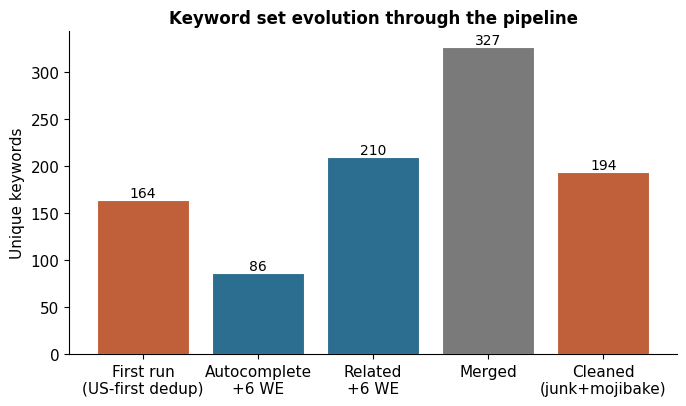
\includegraphics[width=0.8\linewidth]{figures/fig5_funnel.png}
\caption{Evolution of the unique-keyword count through the collection pipeline. The first single-pass run (red) understated non-US regions because of a deduplication ordering artefact. Region-specific related searches recovered genuine cross-country vocabulary; merging and cleaning (junk-term removal and encoding repair) produced the final set of 194 unique keywords.}
\label{fig:funnel}
\end{figure}

The two Google surfaces contribute very differently, as shown in Figure~\ref{fig:source}. Autocomplete, being region-invariant, returned an identical set of 86 unique suggestions regardless of the region code with 540 records that collapse to those 86 strings. Related searches returned 762 records comprising 210 unique keywords, none of which overlapped with the autocomplete set. The autocomplete contribution is small precisely because it is region-invariant: its suggestions largely coincided with the US set and were absorbed during deduplication, whereas each related-search query returns country-specific results. Related searches are therefore solely responsible for the geographic and named-entity richness of the final resource including entities such as \emph{Adriatic Metals}, \emph{Rock Tech Lithium}, \emph{ArcelorMittal Zenica} and \emph{Ržr Ljubija AD Prijedor} appear only through this channel.

\begin{figure}[ht]
\centering
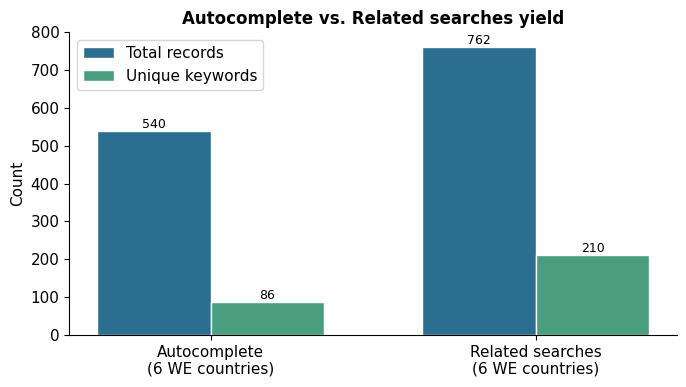
\includegraphics[width=0.8\linewidth]{figures/fig2_source_yield.png}
\caption{Yield of the two collection surfaces for the six Western European regions. Autocomplete produces many records but few unique keywords and no geographic variation; related searches produce the bulk of the unique, region-specific vocabulary.}
\label{fig:source}
\end{figure}

\subsection*{Geographic structure of search demand}

A central empirical finding is that search demand for BiH natural resources is highly redundant across neighbouring European markets. Figure~\ref{fig:overlap} shows, for the 210 related-search keywords collected across the six WE countries, how many countries each keyword is shared by. Only a minority of keywords are unique to a single country (GB 17, AT 10, FR 8, NL 8, IT 7, DE 6), while 47 keywords appear in all six markets simultaneously. The average pairwise overlap between two WE countries is 87 shared keywords. This redundancy is itself a result: interest in Bosnian resources is largely homogeneous across Western Europe rather than fragmented by nation, which is why a single ``Western Europe'' region is a defensible aggregation for downstream use.

\begin{figure}[ht]
\centering
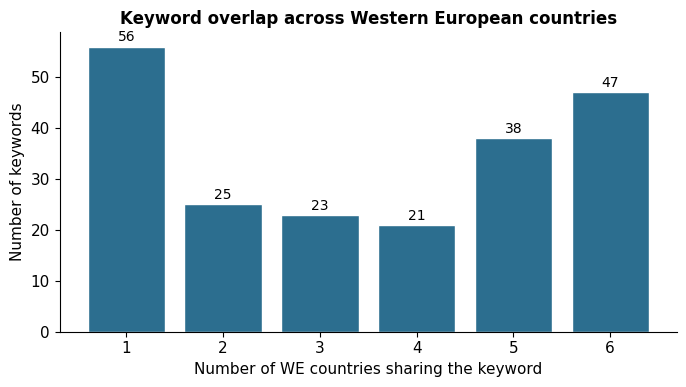
\includegraphics[width=0.8\linewidth]{figures/fig3_we_overlap.png}
\caption{Keyword overlap across the six Western European markets. Each bar counts keywords shared by exactly that many countries. The large mass at six countries and the small single-country tails indicate that demand is broadly shared rather than nation-specific.}
\label{fig:overlap}
\end{figure}

The counts in Figures~\ref{fig:source} and~\ref{fig:overlap} describe the raw related-search collection, before junk removal and cross-set deduplication; the remaining figures describe the final cleaned resource.

After merging the corrected regional collections with the original set and applying cleaning (Methods), the final resource contains 194 unique keywords and 589 (keyword, region) records. Figure~\ref{fig:country} shows the per-region record counts. The distribution is balanced rather than US-dominated (US 116, GB 91, NL 84, DE 82, AT 75, IT 75, FR 66); the residual US lead is expected because the US column retains both its autocomplete and related-search records, whereas the WE records are region-specific related searches. Of the unique keywords, 63 are exclusive to the US region, 78 are exclusive to Western Europe, and 53 are shared, confirming that the region-specific collection recovered substantial vocabulary that the single-pass run had masked.

The final set was reached from an initial single-pass collection of 164 keywords by adding region-specific related searches and applying the cleaning steps described in Methods. The correction changed both the size and the regional composition of the resource.

\begin{figure}[ht]
\centering
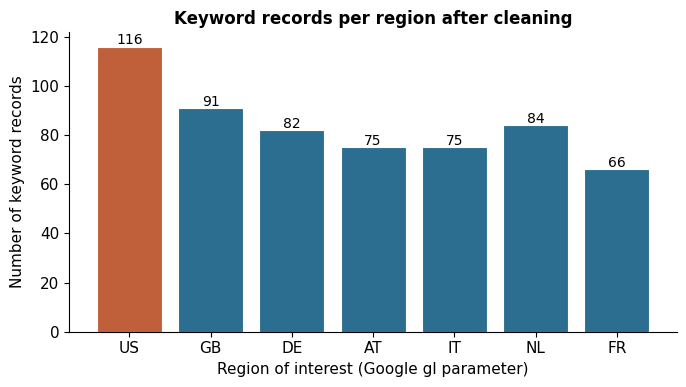
\includegraphics[width=0.8\linewidth]{figures/fig1_per_country.png}
\caption{Keyword records per region of interest in the final cleaned resource. The balanced profile replaces the misleading 73\% US concentration of the single-pass collection.}
\label{fig:country}
\end{figure}

\subsection*{Thematic coverage of the resource}

Grouping the keywords by the resource category of their seed (Figure~\ref{fig:cats}) shows that coverage concentrates on the country's economically salient resources. General and investment-oriented terms are most numerous (39 unique keywords), followed by lithium (32), gas and oil (26) and iron and steel (25). Base metals such as lead, zinc, copper and manganese, together contribute 18, while forestry and timber 15. Less represented categories (water, agriculture) reflect genuinely thin search demand rather than a collection gap. This thematic profile mirrors the public salience of BiH resources, for example lithium prospecting near Lopare and the Zenica steelworks are recurrent news topics and are correspondingly well represented.

\begin{figure}[ht]
\centering
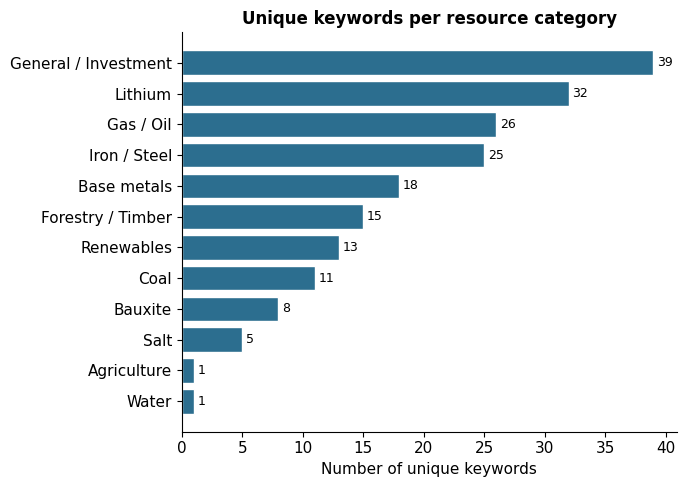
\includegraphics[width=0.85\linewidth]{figures/fig4_resource_cats.png}
\caption{Unique keywords per resource category in the final resource. Coverage tracks the economic and journalistic salience of each resource type.}
\label{fig:cats}
\end{figure}

\subsection*{Corpus, topic annotation and retrieval}

The article corpus is a sample of klix.ba news articles from which 3{,}796 resource-related articles were retained for modelling. Because the portal's native editorial sections are too broad for resource analysis, each article was assigned a fine-grained resource topic by large-language-model annotation into 15 classes (\emph{coal}, \emph{mining}, \emph{oil}, \emph{gas}, \emph{iron\_steel}, \emph{hydropower}, \emph{water\_res}, \emph{forest\_wood}, \emph{lithium}, \emph{base\_metals}, \emph{bauxite}, \emph{salt}, \emph{solar}, \emph{wind}, \emph{agriculture}), which were additionally grouped into four macro-classes (extraction, hydrocarbons, renewables, land-and-water) for coarse analysis. The class distribution is markedly imbalanced, ranging from 960 \emph{coal} articles to 40 \emph{salt} articles. After preprocessing, TF--IDF vectorization with unigrams and bigrams produces the sparse feature matrix used by all downstream components.

Retrieval quality was evaluated with the topic match rate, the proportion of top-$k$ recommended articles sharing the query article's topic, over a fixed random sample of 300 query articles at $k \in \{3,5,10\}$, using the annotated topic as a relevance proxy. Table~\ref{tab:retrieval} reports this rate at the macro-class level for the two set/vector similarity methods. Cosine similarity over TF--IDF vectors is the strongest and most stable method, retrieving a same macro-class neighbour in 88--89\% of cases. Jaccard over binary token sets is consistently a few points lower, as expected for the sparse, specialised vocabulary. Match rate decreases gently with $k$, reflecting the natural dilution of relevance as more neighbours are returned.

\begin{table}[ht]
\centering
\begin{tabular}{lccc}
\toprule
Method & Match rate, $k{=}3$ & Match rate, $k{=}5$ & Match rate, $k{=}10$ \\
\midrule
Cosine (TF--IDF)  & \textbf{0.889} & \textbf{0.878} & \textbf{0.855} \\
Jaccard (tokens)  & 0.863 & 0.855 & 0.833 \\
\bottomrule
\end{tabular}
\caption{\label{tab:retrieval}Retrieval quality by similarity method, reported as the macro-class match rate (share of top-$k$ neighbours in the query's macro-class) over 300 sampled queries. Cosine similarity is strongest at every $k$.}
\end{table}

\subsection*{Topic classification}

As an auxiliary task, the annotated topic was predicted from the TF--IDF representation, both at the fine-grained (15-class) and macro (4-class) levels, under a stratified 75/25 train--test split. Table~\ref{tab:clf} reports the results. At the fine-grained level the task is hard because of strong class imbalance and semantically adjacent topics: Random Forest \cite{breiman2001random} reaches 0.834 accuracy (0.82 weighted F1), well ahead of a Decision Tree (0.736) and Multinomial Naive Bayes (0.449). The low Naive Bayes score reflects its sensitivity to the dominance of the \emph{coal} and \emph{mining} classes. At the macro level all models improve sharply, with Random Forest reaching 0.916 accuracy and 0.898 macro-F1, confirming that most confusions occur within a macro-class rather than across resource types.

\begin{table}[ht]
\centering
\begin{tabular}{lcccc}
\toprule
 & \multicolumn{2}{c}{Fine (15 classes)} & \multicolumn{2}{c}{Macro (4 classes)} \\
\cmidrule(lr){2-3}\cmidrule(lr){4-5}
Classifier & Accuracy & Macro-F1 & Accuracy & Macro-F1 \\
\midrule
Random Forest & \textbf{0.834} & \textbf{0.772} & \textbf{0.916} & \textbf{0.898} \\
Decision Tree & 0.736 & 0.609 & 0.869 & 0.851 \\
Naive Bayes\textsuperscript{$\dagger$} & 0.449 & 0.234 & 0.889 & 0.865 \\
\bottomrule
\end{tabular}
\caption{\label{tab:clf}Topic-classification performance at fine-grained and macro levels, under a stratified 75/25 split. \textsuperscript{$\dagger$}Multinomial Naive Bayes at the fine level; Complement Naive Bayes at the macro level. Random Forest is strongest overall.}
\end{table}

The per-topic confusion pattern of the Random Forest at the fine-grained level is shown in Figure~\ref{fig:cm}. The matrix is strongly diagonal, and the off-diagonal mass concentrates exactly where domain overlap is expected: \emph{mining} is confused with \emph{coal}, \emph{lithium} and \emph{iron\_steel}; \emph{bauxite} and \emph{base\_metals} leak into the generic \emph{mining} class; and \emph{renewables} is split across \emph{hydropower}, \emph{wind} and \emph{solar}. These are label-granularity confusions rather than genuine errors, which is why the macro-level scores are so much higher.

\begin{figure*}[t]
\centering
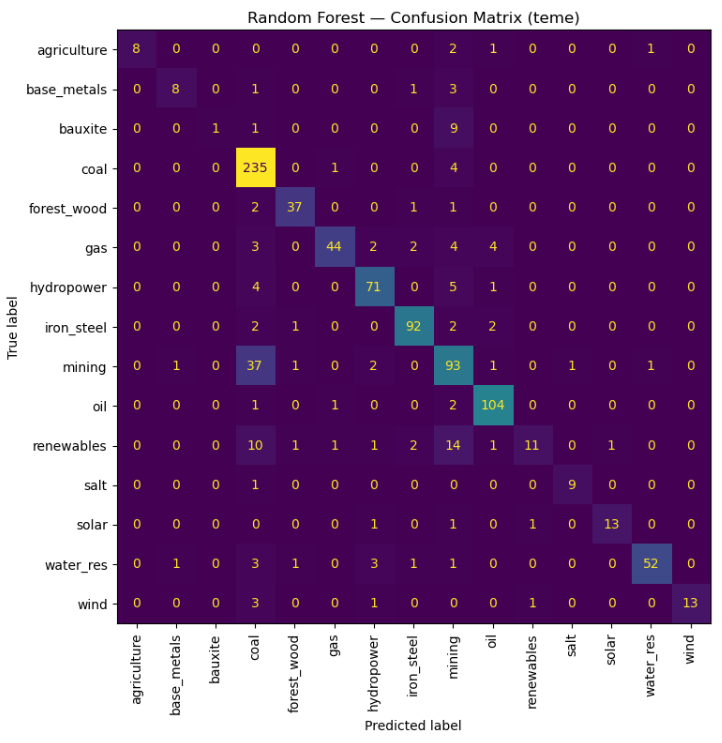
\includegraphics[width=0.78\linewidth]{figures/fig6_confusion_matrix.png}
\caption{Random Forest confusion matrix over the 15 fine-grained resource topics (test split). The matrix is predominantly diagonal; off-diagonal mass falls between semantically adjacent resource classes (e.g. \emph{mining}/\emph{coal}, \emph{renewables}/\emph{hydropower}), which collapse under the macro grouping.}
\label{fig:cm}
\end{figure*}

\subsection*{Deployed application}

The system is delivered as an interactive Django web application. All machine-learning state is built once and held in a cached, in-memory singleton, so that the TF--IDF matrix and fitted models are shared across requests rather than rebuilt per page load. The keyword repository is stored in a relational table and editable through the admin interface. The application exposes six pages.

The \emph{Home} page reports the corpus size, the TF--IDF feature dimensionality and the best-performing retrieval method, framed against the project's predefined success criteria. The \emph{EDA Dashboard} presents the exploratory analysis of the corpus. It incudes topic distribution, article-length and engagement histograms, outlier boxplots and a TF--IDF similarity heatmap over a sample of articles, each rendered as an interactive chart. The \emph{Recommender} page is the direct interface to the three similarity methods: the user selects an article and a metric (cosine, euclidean or Jaccard) and receives its top-$k$ neighbours with their similarity scores, making the differences between metrics visible on real articles. The \emph{Natural Resources} page is the keyword module described above. The user picks a region of interest and one of the selected keywords and the system returns the Bosnian articles most relevant to that keyword via expanded query cosine retrieval. The full keyword repository, grouped by region and showing each keyword's Bosnian expansion terms, is displayed beneath. The \emph{Classification} page shows the fine-grained and macro classifier comparison and the Random Forest confusion matrix for the resource-topic task. The \emph{Demo} page hosts the personalized feed detailed in the Methods and below.

\subsection*{Personalized demonstration feed}

The Demo page illustrates how the recommender behaves as an interactive news feed that adapts to a reader within a single browsing session, using no login and no stored identity. On first visit the reader has no interaction history, so the feed operates in a \emph{cold-start} mode and returns the newest resource articles, already diversified by topic so that the initial feed spans several resource types instead a single dominant one. As the reader clicks articles, each click is recorded against an anonymous session key. From the first click onward the feed switches to a \emph{personalized} mode. It forms a taste profile as the mean of the L2-normalized TF--IDF vectors of the clicked articles, scores every article against this profile by cosine similarity, excludes the already-seen articles and returns the highest-scoring candidates. The profile is therefore a live centroid that shifts with every additional click, so the feed visibly re-orients toward the topics the reader engages with.

Crucially, the ranking is not pure relevance. The candidate pool is re-ranked by the same diversity-aware procedure used throughout, inspired by maximal marginal relevance \cite{carbonell1998use}. A per-topic cap (at most three articles per resource topic) prevents the feed from collapsing onto a single theme even when the profile is strongly peaked; a cumulative similarity penalty, accumulated as each article is selected, suppresses near-duplicate stories while a small recency bonus ranks newer articles upward. The reader can clear their session at any time through a reset control, which deletes the recorded clicks and returns the feed to the cold start state. This page thus makes the whole pipeline tangible. It shows the same TF--IDF representation and cosine scoring that drive the Recommender and Natural Resources pages, now closing the loop into an adaptive, self-diversifying feed.
\section*{Discussion}

The keyword analysis yields a methodological lesson with general applicability. An apparently strong geographic signal in scraped search data can be entirely an artefact of collection order and deduplication granularity. The single-pass run's 73\% US share was not evidence that Americans search more about Bosnian resources, it was the mechanical consequence of iterating the US first and deduplicating on the bare keyword. Only by collecting the one surface that genuinely varies by region—related searches and by deduplicating on the (keyword, region) pair did the true structure emerge and is itself informative. Demand across Western Europe is broadly shared rather than nation-specific, with 47 keywords common to all six markets and an average pairwise overlap of 87 keywords, which justifies treating Western Europe as a single aggregate region.

For the retrieval task, the dominance of cosine similarity over TF--IDF is consistent with the specialised, proper noun-heavy vocabulary of the domain. Exact-term matches on entity names carry most of the signal and bilingual query expansion is what makes an English keyword usable against Bosnian text. The near equivalence of Euclidean and cosine rankings is a direct consequence of L2-normalized vectors and should not be mistaken for two independent methods agreeing.

Several limitations bound these results. The keyword resource is a snapshot of search demand at collection time and will drift as news cycles change. Related search collection is also rate-limited and occasionally returns nothing for a query, so a small number of records were lost to transient failures. The bilingual expansion terms are selected manually, which ensures precision but limits scale and introduces the maintainer's judgement into matching. Finally, the corpus is a sample rather than the full klix.ba archive, so retrieval figures should be read as indicative of method ranking rather than as absolute ceilings.

\section*{Methods}

\subsection*{Keyword collection and cleaning}

Twenty-seven topical seeds were queried through Google Autocomplete and Google Related Searches under seven region codes (US, GB, DE, AT, FR, IT, NL). Related searches were retrieved through a commercial search API \cite{serpapi2024}. Since the free tier is rate-limited, requests used exponential-backoff retries on HTTP 429 responses and a raised read timeout, and results were checkpointed per seed so that a transient failure did not discard collected data. Each returned suggestion was stored as a record of (seed, suggested keyword, source, region).

Cleaning proceeded in a fixed order. First, character encoding repair reversed mojibake introduced when UTF-8 text was read as Windows-1252 (e.g. \texttt{Perućica} $\rightarrow$ \texttt{Perućica}) by re-encoding to cp1252 and decoding as UTF-8. Second, a curated stop list removed off-topic and non-resource suggestions (geopolitical, touristic and unrelated entity queries). Third, deduplication was applied on the (keyword, region) pair. Performing encoding repair before deduplication is essential so that a corrected string and its previously corrupted twin merge into a single record. The resulting resource was persisted with UTF-8 (BOM) encoding to remain robust to spreadsheet reloads.

\subsection*{Query expansion and keyword-to-article matching}

Each keyword is associated with a set of manually selected Bosnian expansion terms that translate the English topic into the vocabulary of the corpus (for example, \emph{bosnia iron ore} expands to \emph{željezna ruda željezo čelik zenica arcelormittal rudnik}). At query time the keyword phrase and its expansion terms are concatenated, projected into the fitted TF--IDF space with the same vectorizer used for the corpus, and scored against every article by cosine similarity and the top-$k$ articles are returned. Expansion is what bridges the language gap, the raw English phrase alone matches Bosnian text poorly, whereas the expansion injects the domain terms that actually occur in the articles.

\subsection*{Text preprocessing and representation}

Article text was lowercased, stripped of digits, punctuation and non-letter characters (retaining Bosnian diacritics \texttt{č ć ž š đ}), whitespace-normalised, tokenized, and filtered against a purpose built Bosnian stopword list that also removes high-frequency journalistic filler (e.g. \emph{prenosi}, \emph{navodi}, \emph{istakao}). Tokens shorter than two characters were discarded. The cleaned documents were vectorized with a TF--IDF model using unigrams and bigrams, a minimum document frequency of two, and a capped vocabulary, producing the sparse matrix used by all retrieval and classification components \cite{salton1988term,jones1972statistical}.

\subsection*{Recommendation pipeline}

The recommender is built in a single offline pass over the article corpus and then queried online. First, each article is reduced to a document string by concatenating its title (weighted twice, by repetition) and body, which biases the representation towards the headline where the most discriminative resource terms occur. These strings are preprocessed (diacritic folding, lowercasing, non-letter stripping, Bosnian stopword removal) and vectorized with a single shared TF--IDF model using unigrams and bigrams, a minimum document frequency of two, a maximum document frequency of 0.5, sublinear term-frequency scaling and L2 row normalization. The resulting sparse matrix $X \in \mathbb{R}^{d \times v}$ ($d$ documents, $v$ vocabulary terms) is the common representation for retrieval, keyword matching and classification, so all three components exist in one consistent space. A parallel binary bin of words matrix $X_{\mathrm{bin}}$ is built with the same tokenizer for the set based Jaccard method.

At query time the recommender exposes a single $k$-nearest-neighbour interface parameterised by the similarity metric. For a query document $i$, the cosine recommender scores every article by the dot product of the L2-normalized rows, $s_j = X_i \cdot X_j$, which equals cosine similarity. The euclidean recommender ranks by $-\lVert X_i - X_j \rVert_2$ and reports the similarity $1/(1+d)$ while the Jaccard recommender scores $|t_i \cap t_j| / |t_i \cup t_j|$ over the binary token sets $t$. In every case the query itself is removed and the top-$k$ remaining articles are returned. Because the TF--IDF rows are L2-normalized, cosine and euclidean rankings are monotonically related and differ only at the margins and Jaccard, operating on unweighted presence/absence, behaves differently and is systematically a few points weaker on this specialised vocabulary.

The keyword-to-article matcher reuses exactly this machinery. A selected keyword and its selected Bosnian expansion terms are concatenated into a pseudo document, transformed by the same fitted TF--IDF vectorizer, and scored against $X$ by cosine similarity. No separate model is trained for the keyword module, actually it is the cosine recommender applied to an expanded query, which is what lets an English search term retrieve Bosnian articles.

\subsection*{Topic annotation}

Because the portal's native editorial sections are far too coarse for resource analysis, resource topics were assigned in a two-stage annotation pipeline. First, a fast lexical pre-filter scanned each article's title and lead using selected Bosnian regular expression patterns inflection, aware term families for each resource class (e.g. \emph{litij}/\emph{lopare}/\emph{Rio Tinto} for lithium; \emph{ugalj}/\emph{ugljenokop}/\emph{termoelektrana} for coal), using to isolate the subset of articles about natural resources and discard the large majority that are not. Second, this candidate subset was passed to a large language model (Qwen3-4B-Instruct) prompted, in Bosnian, to decide whether each article is genuinely about the resource sector and, if so, to assign a single fine-grained topic. The prompt explicitly excludes systematic false positives that the lexical stage cannot distinguish such as sports clubs named after resources (FK Čelik, Rudar), defence and munitions manufacturers and unrelated general industry, so that, for example, an article about a football club called ``Rudar'' is not labelled as mining. Articles the model marked as irrelevant or could not parse were dropped, leaving 3{,}796 annotated articles across 15 fine-grained topics, which were additionally grouped into four macro-classes (extraction, hydrocarbons, renewables, land-and-water). The class distribution is strongly imbalanced, from 960 \emph{coal} to 40 \emph{salt} articles.

\subsection*{Topic classification}

The annotated topic was then treated as a supervised target and predicted from the TF--IDF representation, at both the fine-grained (15-class) and macro (4-class) levels, to test how far the LLM labels are recoverable by a simple classifier. Multinomial (and, at the macro level, Complement) Naive Bayes, a Decision Tree and a Random Forest of 200 trees \cite{breiman2001random} were compared. Only classes with at least 15 examples were kept, and models were trained on a stratified 75/25 split with a fixed random seed and evaluated by accuracy, macro-F1 and, for the best model, a full classification report and confusion matrix.

\subsection*{Evaluation}

Retrieval was assessed with the topic match rate over a fixed random sample of 300 query articles at $k \in \{3,5,10\}$, using the annotated resource topic as a proxy for relevance \cite{lops2011content}. The match rate is reported both at the fine-grained and macro-class levels. The best retrieval method reported on the Home page is the one maximising this rate.

\subsection*{Personalized feed and diversity re-ranking}

The Demo page is served by a separate, session-based recommender operating on a natural-resource article subset. On a cold start (no interactions) it returns the newest articles, diversified by topic. Once a session has clicked articles, it forms a user profile as the mean of the L2-normalized TF--IDF vectors of the clicked articles, scores all articles against this profile by cosine similarity, and re-ranks the candidate pool with a diversity aware procedure inspired by maximal marginal relevance \cite{carbonell1998use}. While the per-topic cap prevents any single resource theme from dominating the feed, a cumulative-similarity penalty discourages near-duplicates and a small recency bonus favours newer articles. Clicks are stored per session key and used only to build the profile.

\subsection*{Implementation and reproducibility}

The application is implemented in Python with Django, scikit-learn, pandas and NumPy. Charts use Matplotlib, Plotly and Seaborn. Fitted pipelines are cached to disk so the models are built once and reused across requests. All random operations use a fixed seed, and the data-preparation and modelling steps follow the CRISP-DM process \cite{wirth2000crisp}. Keyword data flows from a source spreadsheet through a translation step that attaches Bosnian expansions, into a relational store that backs the Natural Resources page.

\bibliography{sample}

\section*{Acknowledgements}

The authors thank the course instructors for guidance on scope and evaluation. Article data originates from the publicly accessible klix.ba news portal and is used for non-commercial academic research.

\section*{Author contributions statement}

T.B. and I.H. jointly designed the system and the keyword-collection methodology. T.B. and I.H. implemented the data pipeline, recommenders and web application, conducted the keyword and corpus analyses, and prepared the figures. Both authors wrote and reviewed the manuscript.

\section*{Additional information}

\textbf{Competing interests.} The authors declare no competing interests.

\end{document}
